\documentclass[12pt]{article}
\usepackage[utf8]{inputenc}
\usepackage[T1]{fontenc}
\usepackage{amsmath}
\usepackage{amsfonts}
\usepackage{amssymb}
\usepackage[version=4]{mhchem}
\usepackage{stmaryrd}
\usepackage{hyperref}
\usepackage{graphicx}
\hypersetup{colorlinks=true, linkcolor=blue, filecolor=magenta, urlcolor=cyan,}
\urlstyle{same}

\begin{document}
These are problems meant to expand upon lecture. 

\section{}
Using the internet for help, sketch the real and imaginary parts of the dielectric function over a $10^0$ to $10^{15} \mathrm{~Hz}$ range for:
\subsection{}
An atom
\subsubsection{Answer}
For a single atom, the only thing we need to consider are electronic excitations.
\subsection{}
A multiple atom molecule
\subsubsection{Answer}
For a multiple atom molecule, we need to consider electronic, vibrational, and rotational excitations.
\subsection{}
A solid
\subsubsection{Answer}
For a solid, we need to consider phonons (vibrational) and electronic excitations.
Acoustic phonons are purely vibrations and optical phonons are when you have a photon coupled to a phonon. The optical phonons are the ones that will have a higher frequency, i.e., higher energy.\\
\begin{figure}[h]
\centering
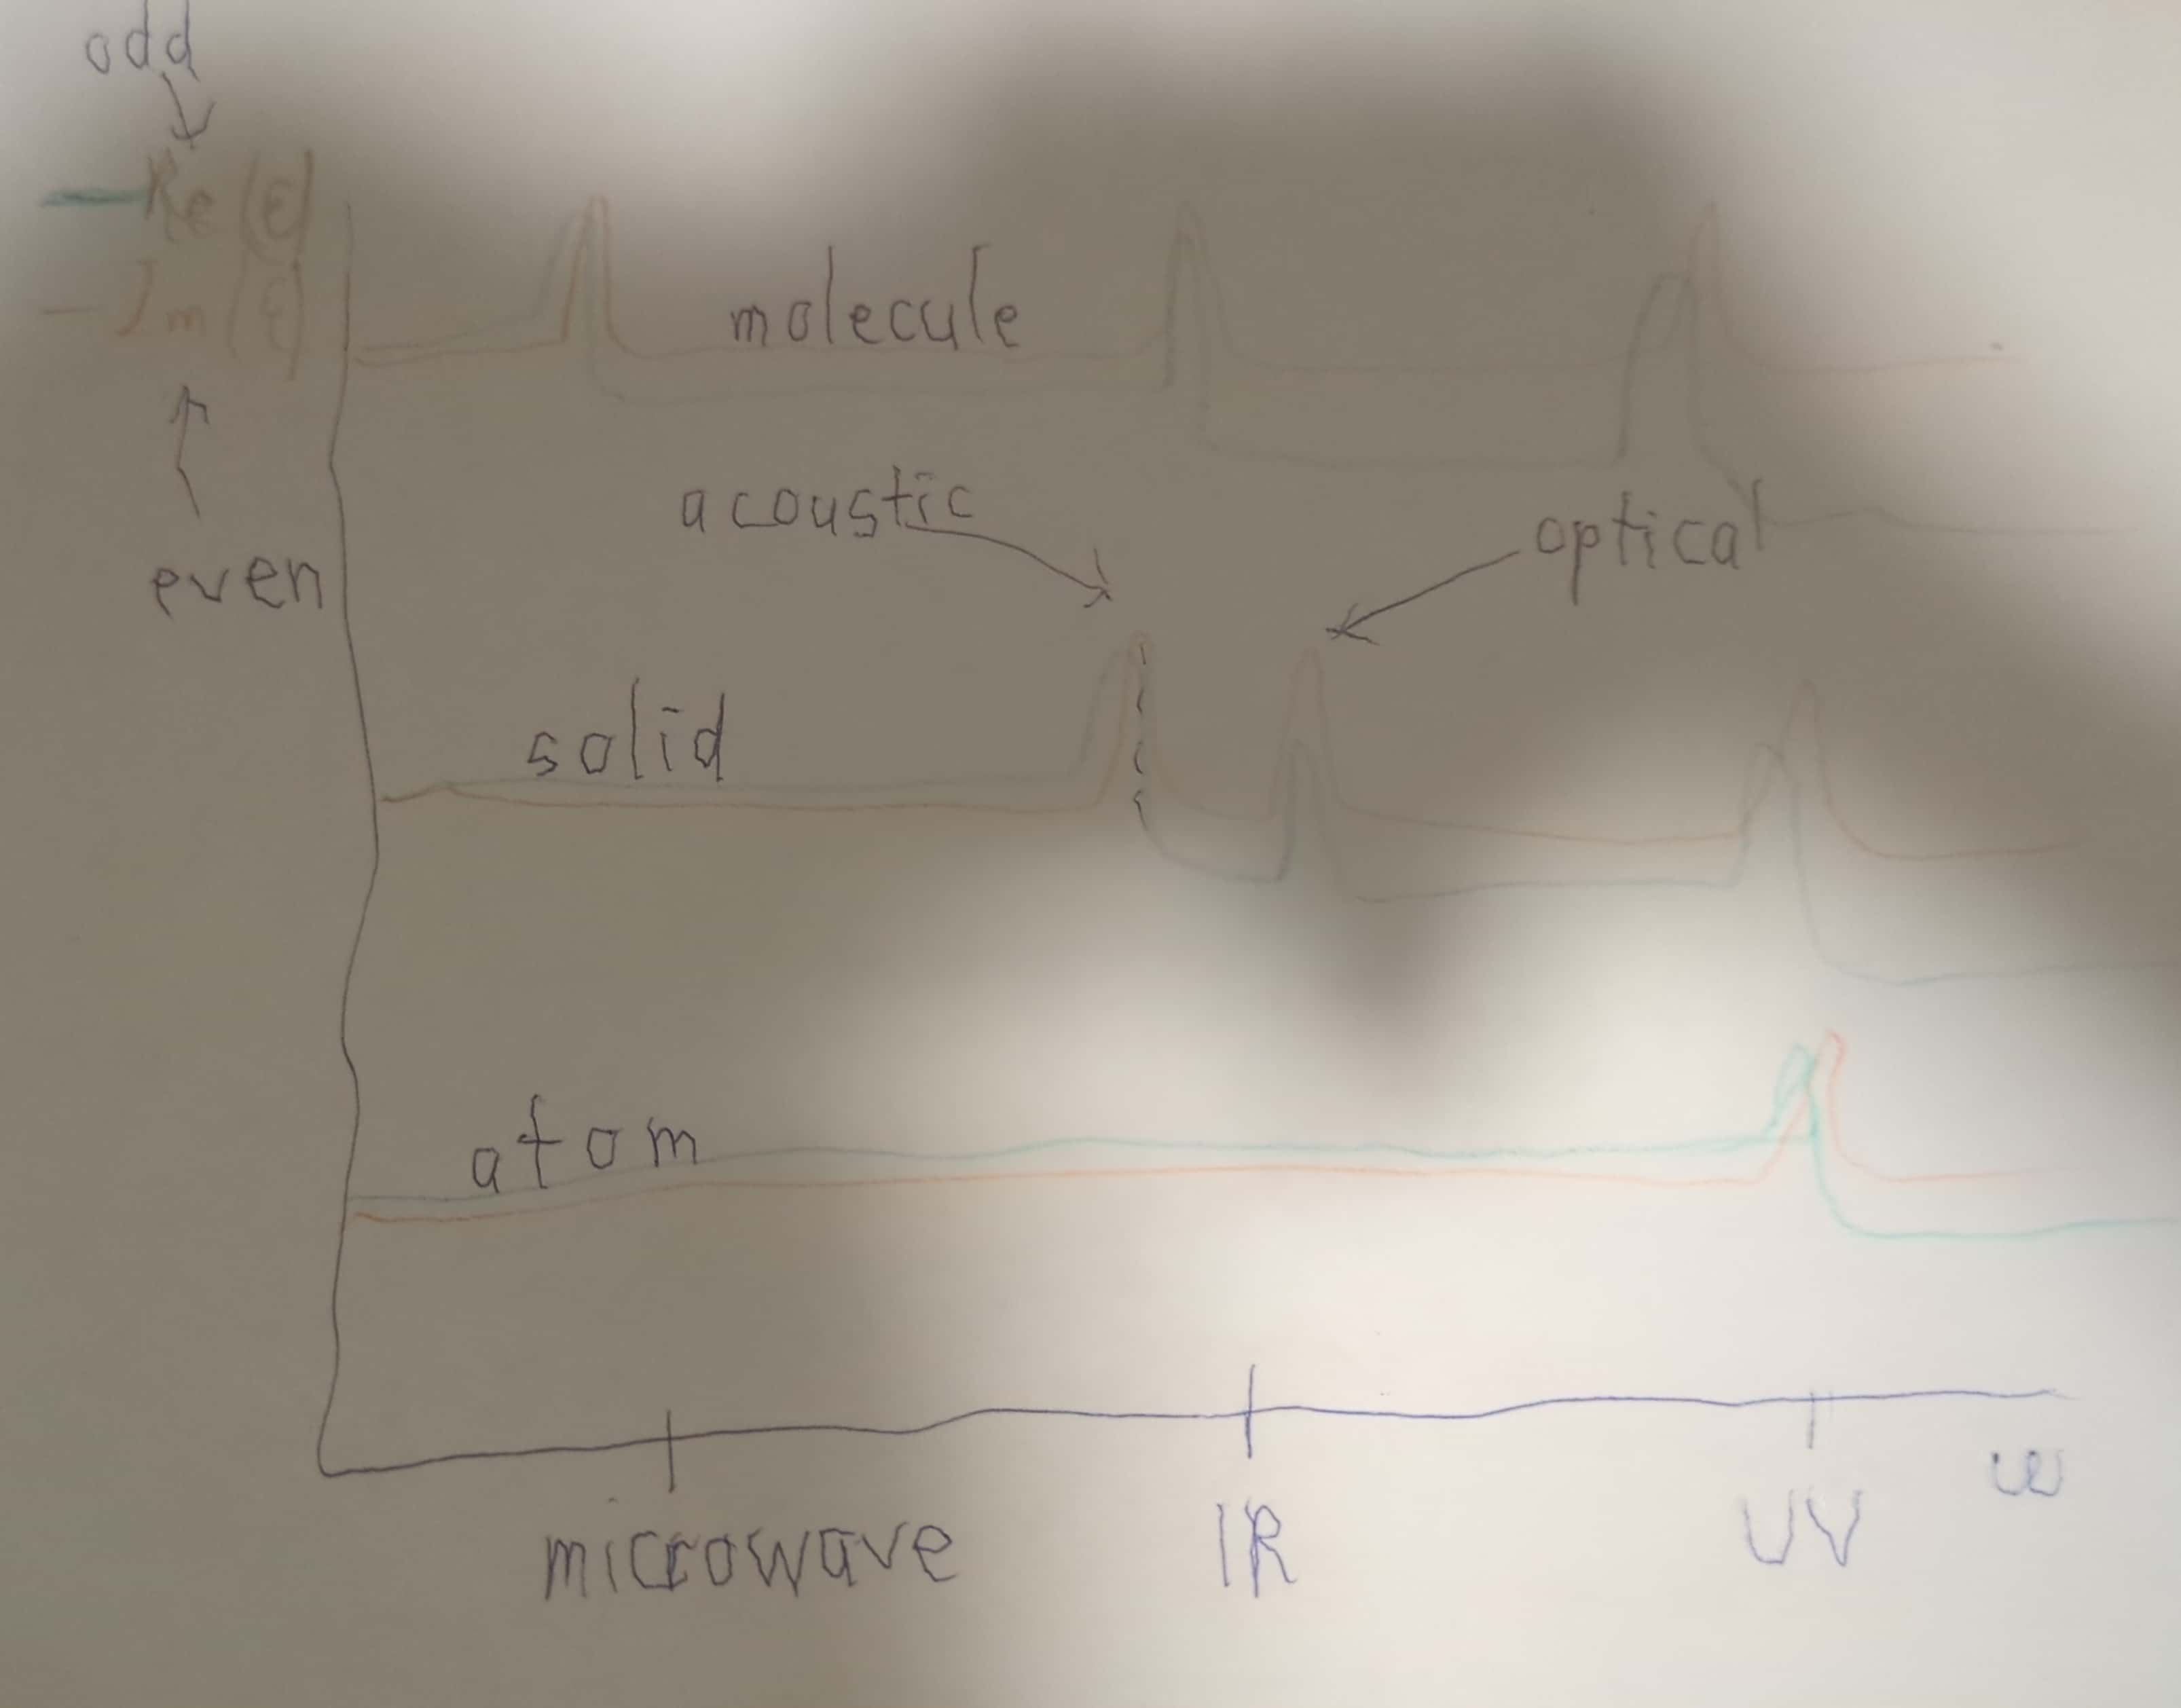
\includegraphics[width=\textwidth]{dielectrics_v2.jpg}
\caption{Dielectric function for an atom, a multiple atom molecule, and a solid.}
\end{figure}
Features do not need to be exact or to scale. Label the key excitations that are present in each system. Hint: What rotational, vibrational, and electronic excitations are possible for each?

\section{}
Dephasing refers to the initial scattering processes that cause the electron-hole pair wavefunction to become out of phase with the driving frequency. Before dephasing a superposition state exists between the excitation and exciting field, i.e. no real population is created. For the same following systems, order them from longest coherence time to shortest. (Hint - e-e scattering goes as the free carrier density and is the fastest, after this it is vibrations, etc)
\subsection{}
An atom
\subsubsection{Answer}
There are no free electrons here to scatter, so the longest coherence time.
\subsection{}
A diatomic species
\subsubsection{Answer}
We have introduced the potential for vibrations so with respect to the single atom, so this will have a slightly shorter coherence time.
\subsection{}
A multiple atom molecule
\subsubsection{Answer}
There are more potential vibrations here with respect to the diatomic, so this will have a slightly shorter coherence time.
\subsection{}
A semiconductor
\subsubsection{Answer}
We have introduced the potential for free carrier electrons here if we have excited across the band gap, so this will have a slightly shorter coherence time than the multiple atom molecule. Phonons are also a possibility.
\subsection{}
A metal
\subsubsection{Answer}
There is no band gap to consider here, so there will be much more scattering between electrons than for the semiconductor. As in the previous case, phonons are also possible.\\
So, the order is: Atom, Diatomic, Multiple Atom Molecule, Semiconductor, Metal.

\section{}

We do not have time to talk about semiconductor junctions in class.
\subsection{}
Research and draw an n-type Metal-Semiconductor Schottky barrier, a p-n junction, and a p-type Metal-Oxide-Semiconductor junction. 
\subsubsection{n-type Metal-Semiconductor Schottky barrier}
So when we excite an electron into the conduction band of the semiconductor, it will relax into the metal. And so holes will move from the metal into the valence band of the semiconductor.
\subsubsection{p-n junction}
For the second junction, just consider the p-type semiconductor undergoing a photoexcitation. Ordinarily, if we just created an electron-hole pair in the p-type semiconductor, it would be short-lived, i.e., we would be dealing with recombination effects. However, the n-type semiconductor provides us with an efficient avenue to prevent these recombination effects because the electron is moving away from the hole as it relaxes along the conduction band into the n-type semiconductor. The intermediate region in which the bands are bending is called the depletion layer, and we will have a net positive charge on the side of the p-type semiconductor and a net negative charge on the side of the n-type semiconductor.
\subsubsection{p-type Metal-Oxide-Semiconductor junction}
\subsection{}
For each junction, draw how photoexcited electrons and holes will move assuming only the semiconductor is photoexcited. Again, use the internet for help.\\



Extended Resource for Problem 3: If you want to calculate this for real in a paper, the freely available AFORS-HET software will calculate band bendings, alignments, photoexcited changes, etc., if you give it basic parameters like the work function, band gap, and dopants.

\href{https://www.helmholtz-berlin.de/forschung/oe/ee/si-pv/projekte/asicsi/afors-het/index}{https://www.helmholtz-berlin.de/forschung/oe/ee/si-pv/projekte/asicsi/afors-het/index}


\end{document}